\chapter{Analysis strategy and optimisation}
\label{ch:stop_ana}
\epigraph{\emph{However beautiful the strategy, you should occasionally look at the results.}}{Winston Churchill}

	%In this chapter the core of this thesis will be presented, namely the search for the direct pair-production of the supersymmetric partner of the top quark in all-hadronic final states using a dataset of $36.1\, \ifb$ \pp\ collisions, at a centre-of-mass energy $\rts = 13$ \TeV, delivered by the \ac{LHC} and collected by the \ac{ATLAS} detector. 
	In this chapter one of the author's main contribution will be presented, namely the analysis strategy, together with the optimisation of the search for the direct pair-production of the supersymmetric partner of the top quark in all-hadronic final states using a dataset of $36.1\, \ifb$ \pp\ collisions at a centre-of-mass energy $\rts = 13$ \TeV. In particular, an excursus on the simplified \ac{SUSY} models considered will be presented in Section~\ref{sec:susysig}; the objects used in both data and \ac{MC} will be discussed in Section~\ref{sec:obj_def}; the selection of the events will be discussed in Section~\ref{sec:evtsel}; an overview of the \ac{SM} backgrounds, and the samples used, will be presented in Section~\ref{sec:SMbkg}; finally, the signal region optimisation strategy will be extensively discussed, as one of the main contribution of the author to the analysis, in Section~\ref{sec:SRs}. 


	%The chapter will be structured as it follows: an excursus on the simplified \ac{SUSY} models considered will be presented in Section~\ref{sec:susysig}; the objects used in both data and \ac{MC} will be discussed in Section~\ref{sec:obj_def}; the selection of the events, together with the key variables used and the optimisation of the regions in which the \ac{SUSY} signals were searched for will be presented in in Section~\ref{sec:evtsel}; the nominal procedure used for the background estimation will be discussed in Section~\ref{sec:bkgest}, with particular focus on the data-driven background estimation in Section~\ref{sec:ddbkgest}; the results, together with their interpretation, will finally be presented in Section~\ref{sec:results}.


	\section{SUSY signals}
	\label{sec:susysig}

		As already introduced in Section~\ref{sec:SUSYPheno}, the signals considered in this work are generated using simplified models, meaning that only the \stop, the \ninoone, the \ninotwo, and the \chinoonepm, are the \ac{SUSY} particles considered. In particular, in such models, either \ninotwo\ or \chinoonepm\ is assumed to be the \ac{NLSP} and, the chargino-neutralino mass splitting $\Delta m(\chinoonepm, \ninoone)$ is assumed to be $1$ \GeV, in accordance with the naturalness argument. This implies that the \chinoonepm\ will promptly decay to $\Wboson^*\ninoone$ , with the \Wboson\ emitted as a virtual particle. The decay products of the so-created virtual \Wboson\ will therefore be low \pt\ objects which will not be reconstructed by the \ac{ATLAS} detector. 

		\subsection{Benchmark processes}

			\begin{figure}[!htb]
				% \begin{center}
				\centering
					\subbottom[$\stop\ra t^{(*)}\ninoone$]{
						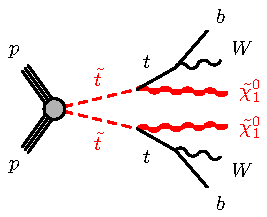
\includegraphics[width=0.28\textwidth]{theory/stst-bqqbqqN1N1-tt}}\hspace{0.05\textwidth}
					\subbottom[$\stop\ra b\ \chinoonepm\ra b \Wboson^{(*)}\ninoone$]{
						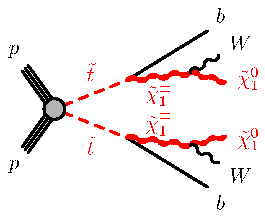
\includegraphics[width=0.28\textwidth]{theory/stst-bbWWN1N1}}\hspace{0.05\textwidth}
					\subbottom[$\stop\ra t\ \ninotwo\to h/Z\ \ninoone$]{
						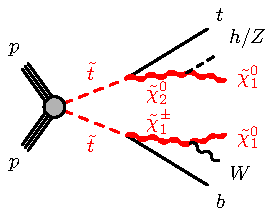
\includegraphics[width=0.28\textwidth]{theory/stst-tbhWN1N1}}\hspace{0.05\textwidth}\\
					\subbottom[$\gluino\ra \stop t$]{
						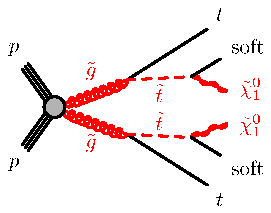
\includegraphics[width=.28\textwidth]{theory/gogo-tsofttsoftN1N1-stst}}
				% \end{center}
				\caption{Diagrams of the decay topologies of the signal models considered in this work.}
				\label{fig:stopModels}
			\end{figure}

			Figure~\ref{fig:stopModels}(a)$-$(c) shows the diagrams corresponding to the decay scenarios considered in this work. In particular, (a) where both top squarks decay\footnote{The symbol (*) indicates off-shell production} via $\stop\rightarrow t^{(*)}\ \ninoone$ (one-step decay); (b) where at least one of the stops decays via $\stop\rightarrow b\ \chinoonepm \rightarrow b\ \Wboson^{(*)}\ \ninoone$ (two-step decay); (c) where $m_{\ninotwo}$ is small enough to allow one stop to decay via $\stop\to t\ \ninotwo \to h/Z\ \ninoone$ where $h$ is the \ac{SM} Higgs boson. Essentially, the experimental signatures searched for in this analysis are characterised by the presence of four or more jets and missing transverse momentum. 

			% \begin{wrapfigure}{R}{.5\textwidth}
			% 	\centering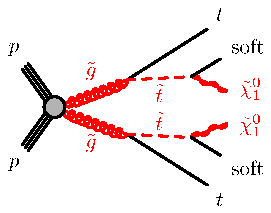
\includegraphics[width=.28\textwidth]{theory/gogo-tsofttsoftN1N1-stst}
			% 	\caption{Diagram of the gluino-mediated top squark production. The term ``soft" refers to decay products whose transverse momenta are below the detector thresholds.}
			% 	\label{fig:gtt}
			% \end{wrapfigure}

			The results of the analysis presented in this and the following chapters were interpreted in the simplified models where only one- and two-step decays scenarios are allowed and, as already mentioned, the latter will be referred to as a natural \ac{SUSY}-inspired mixed grid, \ie\ $\Delta m(\chinoonepm, \ninoone) = 1 \GeV$~\cite{Alwall:2008ve,Alwall:2008ag,Alves:2011wf}. Furthermore, in both scenarios the \ac{LSP} is considered to be a pure bino state. The results will also be interpreted in two slices of the \ac{pMSSM} models: wino-\ac{NLSP} and well-tempered neutralino \ac{pMSSM}~\cite{Djouadi:1998di,Berger:2008cq}.
			A fourth scenario, in addition to direct pair production, was considered: top squarks can also be indirectly produced via gluino decays, as illustrated in Figure~\ref{fig:stopModels}~(d). In such model, the mass difference between the top squark and the neutralino is considered to be relatively small, $\Delta m(\stopone, \ninoone) = 5$ \GeV, allowing the jets originating from \stopone\ decay to have a \pt\ below the reconstruction threshold of the \ac{ATLAS} detector resulting in an experimental signature nearly equivalent to the one in Figure~\ref{fig:stopModels}(a).


		\subsection{MC samples}

			A grid of points across the $(\mstopone-\mninoone)$ plane with a $50$-\GeV\ spacing is generated to simulate the above-mentioned simplified models. %The mixing between the partners of the left- and right-handed top quarks is assumed to be maximal, \ie\ ..
			The signal models were generated using \texttt{MG5\_aMC@NLO 2.2-2.4}~\cite{madgraph} interfaced to \texttt{PYTHIA8}~\cite{pythia8} for the \ac{PS} and hadronisation. \texttt{EvtGen 1.2.0}~\cite{evtGen} was employed for the decays of the  $b$- and $c$-hadrons. The tree-level \ac{ME} calculation includes the emission of up to two additional partons for all signal samples. The \texttt{NNPDF2.3LO} \ac{PDF}~\cite{PDFs} set was used to generate the signal samples with the \verb+A14+~\cite{CT10} tune for the \ac{UE} and shower parameters. Additionally, the \ac{CKKW} prescription~\cite{CKKW} was used for the \ac{ME}–\ac{PS} matching. 

			The various signal cross sections were all calculated to next-to-leading order in the strong coupling constant, with the addition of soft-gluon emission re-summation at next-to-leading-logarithm accuracy (NLO+NLL)~\cite{Beenakker:1997ut, Beenakker:2010nq, Beenakker:2011fu}. The sparticle mass spectra for \ac{pMSSM} models were calculated using \texttt{Softsusy 3.7.3}~\cite{Allanach:2001kg, Allanach:2013kza} while the decays of each sparticle were performed by \texttt{HDECAY 3.4}~\cite{hdecay} and \texttt{SDECAY 1.5/1.5a}~\cite{sdecay}. Finally, various \ac{PDF} sets, factorisation, and re-normalisation scales were used to generate an envelope of cross-section predictions, within which a nominal value and uncertainty were chosen. Further details can be found in~\cite{Borschensky:2014cia}.


	\section{Objects definition}
	\label{sec:obj_def}
			
		The physics objects used in this analysis are obtained using the algorithms discussed in Section~\ref{sec:objReco}. They are required to pass a first loose selection to be categorised as \emph{baseline} objects. An additional procedure is employed to remove potentially overlapping objects, \eg\ a lepton that is identified as a jet, or a lepton that falls within the same jet cone. A so-called \ac{OR} procedure, whose inputs are two baseline objects, is employed to resolve such ambiguities by discarding one of the two objects by looking at their distance ($\Delta R$) and applying some selection criteria, as shown in Table~\ref{tab:OR}. 

		\begin{table}[!htb]\centering\caption{List of the possible ambiguities with relative criteria and decisions.}
		\renewcommand{\arraystretch}{1.3}
			\begin{tabular}{lccc}
				\toprule 
				\textbf{Ambiguity} & \textbf{Criterion} & \textbf{Object kept} & \textbf{Object removed}\\
				\toprule
				\multirow{2}{*}{electron/jet} & $\Delta R (e,\mathrm{jet}) < 0.2$ & electron & jet\\
				& $0.2 \leq \Delta R (e,\mathrm{jet}) < 0.4$ & jet & electron \\\midrule
				electron/\bj & $\Delta R (e,\bj) < 0.2$ & \bj\ & electron\\ \midrule
				\multirow{2}{*}{muon/jet} & $\Delta R (\mu,\mathrm{jet}) < 0.4$ and & \multirow{2}{*}{muon} & \multirow{2}{*}{jet} \\ 
						& $N_{\mathrm{tracks}} < 3$, $\pt^{\mathrm{track}} > 500$ \MeV &  &  \\ \midrule
				photon/electron & $\Delta R (e,\gamma) < 0.4$ & electron & photon\\ 
				photon/muon & $\Delta R (\mu,\gamma) < 0.4$ & muon & photon\\ 
				photon/jet & $\Delta R (\mathrm{jet}, \gamma) < 0.4$ & jet & photon\\ 
				\bottomrule
				\end{tabular}
				\label{tab:OR}
		\end{table}

		The data-driven estimation of \ttZ\ events using \ttgamma\ (discussed in Section~\ref{sec:ddbkgest}) is the only part of the analysis that used reconstructed photons. In particular, the \ac{OR} is modified accordingly to avoid that an object will appear in multiple collections (double-counting). The various baseline and signal objects are defined as:

		\begin{description}
			\item[Electrons] 
				baseline electrons are required to have $\abseta < 2.47$, $\pT > 7$ \GeV\ and have to pass a \texttt{VeryLoose} likelihood-based selection (further details in~\cite{egamma, egamma2}). Electron candidates which pass the \ac{OR}, have a $\pt > 20$ \gev\ ($\pt > 28$ \GeV) in events selected with a \met\ (lepton) trigger, satisfy $d_0/\sigma_{d_{0}} < 5$, $z_0 \sin \theta < 0.5$, and pass a \texttt{Tight} likelihood-based selection isolation, are identified as ``signal'' electrons;

			\item[Muons] 	
				baseline muons have to pass a \texttt{Loose} selection~\cite{PERF-2015-10}, satisfy $\abseta < 2.7$ and $\pt > 6$ \GeV. Further requirements are imposed on muon candidates to tag them as signal. In particular, they have to pass the \ac{OR}, a \texttt{Medium} quality selection~\cite{PERF-2015-10}, and satisfy
				$|d_0|< 3 \sigma_{d_0}$ and $|z_0 \times \sin \theta |<0.5$. Additionally, the \pt\ requirement is tightened up to $20$ \gev\ ($28$ \GeV) in regions with a \met\ (lepton) trigger;

			\item[Photons]
				baseline photons have to pass a \texttt{Tight}~\cite{Aaboud:2016yuq} selection, and have $\pt > 25$ \GeV\ and $\abseta < 2.37$. Additionally, baseline photon candidates are required to have $\pt > 130$ \GeV\ and satisfy a tighter isolation selection, in order to be tagged as signal;
			
			\item[Jets]
				as already mentioned in Chapter~\ref{sec:objReco}, jets are reconstructed using the \antikt\ algorithm with $R=0.4$. Baseline jets are required to have $\pt>20$ \GeV\ and $\abseta< 4.8$. Signal jets have to pass the \ac{OR}, satisfy the \ac{JVT} requirement, and have $\abseta < 2.8$ and $\pt > 20$ \GeV. 

			\item[b-tagged jets]
				baseline jets in the event are identified as originating from the decay of a $b$-quark is based on the \texttt{MV2c10} jet tagger which uses the a $77\%$ fixed-cut WP. The \pt\ threshold applied to signal jets is also applied to \bj\ and the requirement on the pseudorapidity is relaxed down to $\abseta < 2.5$.
			
			\item[Missing transverse energy]
				The \met\ is reconstructed as described in Section~\ref{sec:objReco}. Baseline muons, electrons, and jets after overlap removal are used in the \met\ recalculation. 
				% The \textit{soft} term in the event, already introduced in Section~\ref{sec:objReco}, that is not associated with any of the selected objects is calculated from inner detector tracks with $\pt > 400$ \MeV\ matched to the \ac{PV} to make it more resilient to pileup contaminations. 

				Additionally, in the analysis carried out during Run-1~\cite{stop0LRun1} another \met-related quantity was introduced. The track-based \met, derived from the sum of the \pt\ of the tracks associated with the objects in the event was found to have discriminating power to reject fake \met. The \ptmisstrk, whose magnitude is \mettrk, from the tracking system is computed using the vector sum of the reconstructed inner detector tracks, $\ptmisstrk = \sum_i^{\mathrm{tracks}} \pt^i$, with $\pT > 500$ \MeV\ and $\abseta < 2.5$, that are associated with the \ac{PV} in the event. 
 		\end{description}

		Ultimately, leptons are also required to satisfy \pt-dependent track- and calorimeter-based isolation criteria. The calorimeter-based isolation is determined by taking the ratio of the sum of energy deposits in a cone of $R = 0.2$ around the electron or muon candidate and the energy deposits associated with the electron and muon. The track-based isolation is estimated in a similar way but using a variable cone size with a maximum value of $R = 0.2$ for electrons and $R = 0.3$ for muons. An isolation requirement is made that is $95\%$ efficient for electron or muon candidates with $\pt = 25$ \GeV\ and $99\%$ for candidates with $\pt = 60$ \GeV.

		
	\section{Triggers used}

		As previously discussed in Chapter~\ref{ch:detector} and~\ref{ch:trigger}, physics events are recorded once they passed a certain trigger. In particular, a \met\ trigger is used to select events that fall in signal-enriched regions, \ac{SR}, where no leptons, but jets and missing \et\ are required; a single-lepton (or photon) trigger is used to select events in background-enriched regions, where $1$-lepton (or photon) is required. A breakdown of all the lowest unprescaled online triggers used will be presented below.

		%\begin{description}
			Once the \met\ is reconstructed from an input jet collection, events are selected with a missing \et\ trigger by selecting a $70$-\GeV\ threshold in the $2015$ dataset whereas, due to the increase in instantaneous luminosity (impact on the trigger rate), in $2016$ the threshold was gradually raised to $90$, $100$, and $110$ \GeV. It can be seen (Figure~\ref{fig:mettrigger}) that for analysis purposes a cut of at least $200$ \GeV\ is required to stay in a region where the trigger is fully efficient (\emph{plateau}); 

			Events are selected with a single-electron trigger by using a logic \texttt{OR} of three electron-trigger chains: the first consists of a $24$-\GeV\ threshold ($26$-\GeV\ in $2016$ data); the second chain uses a $60$-\GeV\ threshold without additional isolation requirement; the third uses a $120$-\GeV\ threshold to be efficient at high \et. A $\pt^e > 27$ \GeV\ cut is applied to both $2015$ and $2016$ datasets to stay in the plateau region;

			Events are selected with a single-muon trigger by using a logic \texttt{OR} of two chains: a first chain with a $20$-\GeV\ threshold is used in data $2015$ and $26$-\GeV\ threshold, together with an isolation requirement, in $2016$; a second chain with a $50$-\GeV\ threshold is employed for both $2015$ and $2016$ data. A $\pt^\mu > 27$ \GeV\ is applied to both $2015$ and $2016$ datasets to stay in the plateau region;

			Events are selected with a single-photon trigger by using only one chain: a $120$ \GeV\ ($140$ \GeV) threshold is employed in $2015$ ($2016$). Additionally, in order to ensure full trigger efficiency a $\pt^\gamma > 150$ \GeV\ cut is applied.
		%\end{description}


	\section{Event selection}
	\label{sec:evtsel}

		A cut-and-count strategy is at the heart of the analysis presented here. Dedicated sets of discriminating variables are employed to isolate, where possible, the targeted signals from the main \ac{SM} backgrounds. Equally, background-enriched regions are defined to \emph{control} the modelling of such backgrounds. The number of events passing such selections is used as the main observable, to predict both signal and background processes either by means of \ac{MC} samples, or using data-driven techniques. In general, a combination of the two is employed. 

		The \ac{ATLAS} detector did not operate with the same conditions during $2015$ and $2016$: different triggers, and calibration parameters were used. In order for \ac{MC} parameters to be modified consistently with what is done in data, \ac{MC} events are assigned a random number, which identifies an ATLAS run. This procedure provides consistency between the collected data and the simulated \ac{MC} events. %to be associated with specific data-taking periods such that their parameters are associated what is done in data and can be modified accordingly.

		\subsection{Event cleaning}

			In order to remove events where the a detector fault might have occurred, a set of offline cuts is applied to clean the used event sample. The first requirement for an event to be a good physics event is the existence of a primary vertex with a minimum of two tracks, with $\pt\ > 400$ \MeV, associated with it. In addition, the status of both \ac{ECAL} and \ac{HCAL} for that event is checked: if any of the calorimeters returned an error state, the event is discarded. Furthermore, to reduce and suppress the fake-jet contamination a \emph{bad jet} requirement is defined by introducing quality requirements on a variety of jet parameters, \eg\ the fraction of energy deposited in the different layers of the calorimeters, and the fraction of jet \pt\ measured by the tracks in the Inner Detector. Events containing bad jets that passed the \ac{OR} are discarded. Similarly, events containing baseline muon candidates, whose relative uncertainty on $e/p$ is larger than $20\%$, and which were found before the \ac{OR}, are discarded. This also applies to events containing those potentially cosmic muons which were not removed by the \ac{OR}.				


	\section{Standard Model backgrounds}
	\label{sec:SMbkg}

		As already anticipated in Section~\ref{sec:SMlim}, there exists a wide variety of \ac{SM} processes whose cross sections are significantly larger than \ac{SUSY} signal ones. In order for the analysis to robustly target the desired signal, the accurate modelling of such backgrounds is a fundamental part. The signal region definitions, whose modelling is strictly related to the sensitivity reached by the analysis, need an accurate knowledge of the kinematical properties of both targeted signals and backgrounds. The backgrounds which contribute to the search of direct stop-pair production in final states with jets and \met, with their relative \ac{MC} samples employed, will be discussed below.

		\begin{description}

			\item [Top pair production:] \ttbar\ production is a major background for many third-generation \ac{SUSY} analyses at the LHC. The dominant top-quark decay is $t \to b \Wboson$ with a \ac{BR} of $\sim 99.8\%$, which in turn yields two oppositely charged \bjs\ and \Wboson\ bosons. These will then yield $0$-lepton, $1$-lepton, and $2$-lepton final states, with $45.7\%$, $43.8\%$, and $10.5\%$ \acp{BR} respectively, giving the name to the fully hadronic, semi-leptonic, and di-leptonic \ttbar\ decays, respectively; 
			
			\item [Single top production:] the production of one single top is also possible at the LHC. The different decays are usually referred to as $s$-channel, $t$-channel, and $\Wboson\ t$ channel, the last one being the most relevant for this analysis since it yields a \Wboson; 

			\item [$\mathbf{\Zboson}$ boson production in association with jets:] the production of a \Zboson\ boson in association with jets is a major backgrounds in both $0$-lepton plus \met\ and $2$-lepton final states because of the $\Zboson \to \nu \nu$ and the $\Zboson \to \ell \ell$ decays\footnote{$\ell = e,\mu,\tau$}, with a \ac{BR} of $\sim 20\%$ and $\sim 10\%$, respectively. Although the hadronic decay of the \Zboson\ boson ($\Zboson \to qq$) has the largest \ac{BR} ($\sim 70\%$), this is not relevant for third-generation \ac{SUSY} searches, as the multi-jet background dominates. The \Zjets\ \ac{MC} samples are generated categorising\footnote{Using the information at truth level} the events depending on the flavours of the hadrons produced in association with the \Zboson\ boson:
			\begin{itemize}
				\item $b$-filtered: containing at least one $b$-hadron;
				\item $c$-filtered: containing at least one $c$-hadron (no $b$-hadrons);
				\item light-filtered: no $b$- or $c$-hadrons included;
			\end{itemize} 
			In this analysis the major contribution to such background comes from the $b$-filtered sub-sample as the selected events contain \bjs;

			\item [$\mathbf{\Wboson}$ boson production in association with jets:] the production of \Wboson bosons in association with jets is a relevant background in $1$-lepton final states, due to the $\Wboson \to \ell\nu$ decay which has a \ac{BR} of $\sim 32\%.$ The dominant hadronic decay of the \Wboson, $\Wboson \to qq'$, produces a multi-jet final state which, again, is irrelevant for this analysis. The \Wjets\ samples are equally categorised depending on the flavour of the hadrons produced in association with the \Wboson boson;

			\item [Di-bosons production:] albeit the production of pairs of bosons, \Wboson\Wboson, \Wboson\Zboson, and \Zboson\Zboson, can also be a source of background in channels with leptons or jets, depending on the decay mode of each boson;

			\item [Top pairs production in association with a vector boson:] the cross section of the production of top pairs in association with a vector boson or a Higgs boson is smaller than the other processes considered so far. Nevertheless, such background can be a prominent background for third-generation \ac{SUSY} analyses. In particular, the top-pair production in association with a \Zboson\ boson, with the \Zboson\ boson decaying to neutrinos, $\ttZ \to \nu \nu$, does represent an irreducible background for this analysis: it yields a final state with jets and \met\ which looks identical to the signal searched for. For such reason a data-driven technique is employed, where essentially the top-pair production in association with a photon \ttgamma\ is used instead. Further details on the method for its estimation will be given in Section~\ref{sec:ddbkgest}; 

			\item [Multi-jet:] the multi-jet production is the process with the highest cross section among the ones mentioned so far, and even though such events do not contain neither leptons nor \met\ they could resemble the signal due to either isolated but mis-reconstructed leptons or large measured \met\ due to detector resolution. Despite the low probability of such occurrence, the high rate of such background might generate a non-negligible contribution;
		\end{description}

		\noindent For most of the listed backgrounds, a set of additional sub-samples is generated in order to estimate the theoretical uncertainties associated with the generation of the process. The variations of, re-normalisation, factorisation, \ac{CKKW} matching scales, different \ac{PDF} sets or hadronisation models, are included.

		\subsection{MC samples}
		\label{subsec:mc_samples}

			\ac{SM} background samples are generated using different \ac{MC} event generators: the production of \Zjets\ and \Wjets\ events are generated with \textsc{Sherpa}~\cite{Sherpa} using the \verb+NNPDF3.0NNLO+~\cite{PDFs} \ac{PDF} set and the \ac{UE} tune provided by \textsc{Sherpa} itself~\cite{Sherpa}l; \ttbar\ and single-top production are simulated with \textsc{Powheg-Box}~2~\cite{powheg-box} and interfaced to \textsc{Pythia}~\cite{Pythia2006} for \ac{PS} and hadronisation, with the \verb+CT10+~\cite{CT10} \ac{PDF} set. {\scshape MG5\_aMC\/@NLO} interfaced to \textsc{Pythia} for \ac{PS} and hadronisation is used to generate the \ttbar+$V$ and \ttbar+$\gamma$ samples at \ac{NLO} with the \verb+NNPDF3.0NLO+ \ac{PDF} set. The underlying-event tune used is \verb+A14+ with the \verb+NNPDF2.3LO+ \ac{PDF} set. For the estimation of \ttZ\ via $\ttgamma$, $\Wboson/\Zboson+\gamma$ processes are generated with \textsc{Sherpa}~\cite{Sherpa} using the \verb+CT10+ \ac{PDF} set, and finally, the same procedure is used for the generation of di-boson production events.


	\section{Signal Regions optimisation}
	\label{sec:SRs}

		The experimental signature for all signal topologies described in Section~\ref{sec:susysig} is essentially characterised by the presence of multiple jets, two of which are required to have passed the $b$-tagging selection, a significant amount of missing transverse momentum, and no leptons (electrons or muons).

		An initial overview of the five different sets of \acp{SR}, \SRA\ (SRA) to \SRE\ (SRE), employed to target each topology and kinematic regime, is given below: 
		
		\begin{description}
			\item [SRA] is sensitive to the production of high-mass \stop\ pairs with a large \stop--\ninoone\ mass splitting \dmstopnino. It is optimised using a signal point defined by: $(\mstopone, \mninoone) = (1000,1)$ \GeV\ signal point;
			
			\item [SRB] targets decays involving top squarks with high stop mass but with smaller \dmstopnino. It is optimised using signal points defined by:  $(\mstopone, \mninoone) = (700, 400)$ \GeV, and $(\mstopone, \mninoone) = (600, 300)$ \GeV;
			
			\item [SRC] is designed for the so-called highly compressed region where, $\dmstopnino \sim m_t$ and it employs an \ac{ISR} to improve sensitivity to such decays. It targets various signal points \eg\ $(\mstopone, \mninoone) = (500, 327)$, and $(\mstopone, \mninoone) = (300, 127)$ \GeV; 
			
			\item [SRD] targets the $\stopone \to b \chinoonepm$ decay, with $\mchinoonepm = 2\mninoone$, where no top-quark candidates are reconstructed. It is optimised using signal points defined by: $(\mstopone, \mninoone) = (400,50)$ \GeV\ and $(\mstopone, \mninoone) = (700,100)$ \GeV; 
			
			\item [SRE] is sensitive to highly boosted scenarios that can occur in gluino-mediated stop production and it is optimised using signal points defined by: $(\mgluino, \mstopone, \mninoone) = (1700, 400, 395)$ \GeV;
		\end{description}

		\subsection{Preliminary selection and discriminating key variables}
		\label{sec:vars_used}

			A \emph{pre-selection}, essentially a basic selection of candidate events common to all the \acp{SR}, is performed by applying trigger and event-cleaning cuts together with the requirement of a relevant set of physics objects according to the targeted experimental signature. The physics objects, reconstructed as discussed in Section~\ref{sec:objReco}, are used to build the various variables used to discriminate the \ac{SUSY} signal from the \ac{SM} background. The event selection is based on such variables some of which will be described below:

			\begin{description}
				\item[\boldmath $\HT$:] the scalar sum of the \pt\ of all signal \antikt\ $R=0.4$ jets;

				\item[$\dphijettwomet$:] the difference in $\phi$ between the two leading jets (ordered in \pt) and \ptmiss. This variable provides a good rejection of events containing fake \met\ originating from \ac{QCD}, hadronic \ttbar, and detector resolution effects;

				\item[\boldmath $\mtjetimet$:] the transverse mass (\mt) between the $i^{\mathrm{th}}$ jet and the \met\ in the event\\
					% A massless approximation is used for this and all following \mt\ variables:\\
				\begin{center}
					$\mtjetimet = \sqrt{2\ptjeti\met\left[1-\cos{\Delta\phi\left(\mathrm{\mathbf{\ptjeti}},\ptmiss\right)}\right]}$,
				\end{center}
				where $\ptjeti$ is the transverse momentum of the $i^{\mathrm{th}}$ jet;

				\item[\boldmath $\mtbmin$:] transverse mass between closest $b$-jet to $\met$ and $\met$. This variable provides very good discrimination between signal and semi-leptonic \ttbar\ background;

				\item[\boldmath $\mtbmax$:] transverse mass between farthest $b$-jet to $\met$ and $\met$. This variable provides very good discrimination between signal and semi-leptonic \ttbar\ background;
												
				\item[\boldmath $\drbb$:] the angular separation between the two jets with the highest MV2c10 weight. This variable provides additional discrimination against background where the two jets with highest b-tagging weights originate from a gluon splitting;

				\item[\boldmath $\mttwo$]: the stransverse mass. This is built using direction and magnitude of the \ptmiss\ in the transverse plan and the direction of two top-quark candidates reconstructed using a $\chi^2$ method. The minimisation is done in terms of a so-called $\chi^2$-like penalty function $$\chi^2 = \left(m_{\mathrm{cand}} - m_{\mathrm{true}}\right)^2 / m_{\mathrm{true}},$$ \noindent where $m_{\mathrm{cand}}$ is the candidate mass and $m_{\mathrm{true}}$ is set to $80.4$ \GeV\ and $173.2$ \GeV\ for \Wboson\ candidates and top candidates, respectively. First, \Wboson\ boson candidates are formed by using single or pairs of \antikt\ $R = 0.4$ jets, and then combined with additional \bjs\ in the event to construct the top candidates. These, selected by the $\chi^2$ method, are only used for the momenta in \mttwo. The mass hypotheses are set to $173.2$ \gev\ and $0$ \gev\ for the top quarks and the invisible particles, respectively.	Further details on \mttwo\ can be found at~\cite{Barr:2003rg, LESTER199999}.

			\end{description}

			A summary of the pre-selection cuts is shown in Table~\ref{tab:SRcommon}, where three groups of cuts are listed: the first, a \met\ cut of $250$ \GeV, to stay in a region where the trigger is fully efficient, as already mentioned in Section~\ref{sec:evtsel}. The second, a lepton veto\footnote{The event must contain exactly $0$ baseline electron candidates and $0$ baseline muon candidates}, together with a cut on the number of jets (at least four, ordered in $\pt > 80,\,80,\,40,\,40$ \GeV), at least one of which must be b-tagged, as signal events tend to have more energetic jets than the background, to select hadronic \ttbar\ events. The third, an angular separation between the azimuthal angle of the two highest-\pt\ jets and the \ptmiss, to reject events with mis-measured \met\ originating from \ac{SM}-background decays. In addition, in order to further reject these events, a requirement on \ptmisstrk\ to be aligned in $\phi$ with respect to the \ptmiss\ calculated from the calorimeter system, is employed. 
			%multi-jet and hadronic \ttbar\ decays.

			\begin{table}[htbp]
			\caption{Selection criteria common to all \acp{SR} in addition to the event cleaning.}
				\begin{center}
				\renewcommand{\arraystretch}{1.4}
				    \begin{tabular}{lc} 
				    	\toprule
				    	\textbf{Object} & \textbf{Selection} \\
				    	\toprule
				    	Trigger & \met \\ 
					   % & \\ [-2ex] 
					   $\met$ & $> 250\GeV$ \\ 
					   %& \\ [-.5ex] 
					   \midrule
					   $N_{\mathrm{lep}}$ & $0$ \\ 
					   \antikt\ $R=0.4$ jets & $\ge 4,~\pt>80,80,40,40 \gev$ \\ 
					   $b$-tagged jets & $\ge1$ \\ \midrule
					   $\dphijettwomet$ & $> 0.4$ \\ 
					   % & \\ [-2ex] 
					   $\mettrk$  & $> 30 \gev$ \\  
					   % & \\ [-2ex] 
					   $\dphimettrk$ & $<\pi/3$ \\
					   \bottomrule
				    \end{tabular}
					\end{center}
			\label{tab:SRcommon}
			\end{table}

			% \begin{wrapfigure}{R}{.6\textwidth}
			% 	\centering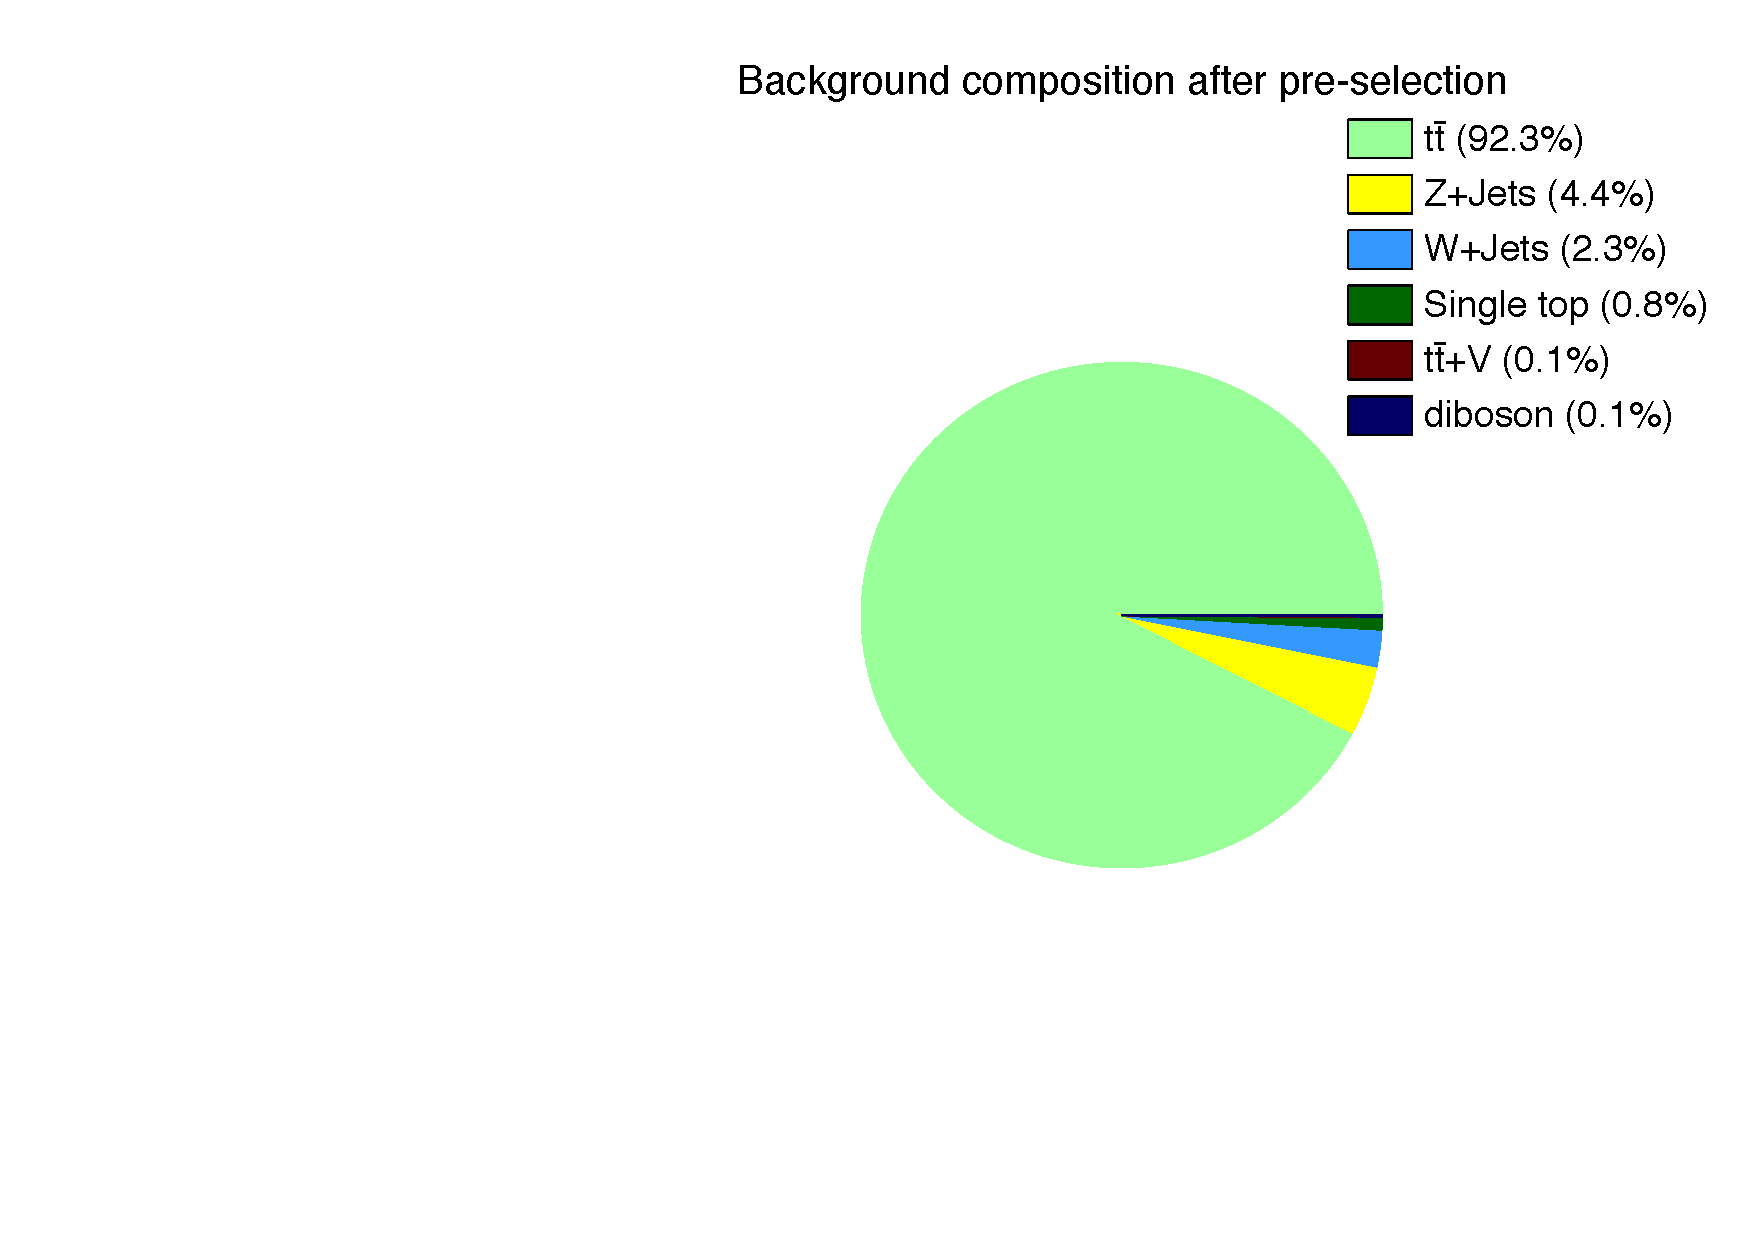
\includegraphics[width=.6\textwidth]{stop/piechart_presel}
			% 	\caption{Pie chart of the background composition after the pre-selection selections described in Table~\ref{tab:SRcommon}}
			% 	\label{fig:piechart_presel}
			% \end{wrapfigure}

			% Figure~\ref{fig:piechart_presel} displays a pie chart of the \ac{SM} background composition, after having applied all the cuts listed in Table~\ref{tab:SRcommon}. The main background is all-hadronic \ttbar\ production, as a result of the requirement on the number of jets and at least $1$ \bj. The \ttbar\ \ac{MC} sample used here is an inclusive sample\footnote{The sample takes into account all the possible \ttbar\ decays: fully hadronic, semi-leptonic and di-leptonic}.
			% % the semi-leptonic and the di-leptonic \ttbar\ decay would be negligible as a lepton veto is applied.



			\paragraph*{Top quark mass reconstruction}

				In addition to the above-mentioned variables, another set of variables is needed to select \acp{SR} targeting the pair production of $\stopone \to t + \ninoone$: the reconstruction of two hadronically decaying top quarks in the event using the jet \emph{re-clustering} algorithm, performed using the \antikt\ algorithm (with a larger distance parameter $R = 1.2$), fed with the calibrated \antikt\ $R = 0.4 $jet collection (further details can be found in~\cite{Antikt2008}). The highest- (second-highest) \pt\ re-clustered jet is chosen to be the first (second) top candidate. The best signal sensitivity is reached by using $R = 1.2$ and $R = 0.8$, for top and \Wboson\ candidates, respectively~\cite{stop0L,ICHEPstop0L}. The variables used are the masses of the $R=1.2$ and $R=0.8$ leading and sub-leading jets, indicated by \mantikttwelvezero, \mantikttwelveone, \mantikteightzero, \mantikteightone, respectively. Such variables help reduce the \ac{SM} backgrounds. %from QCD, \Wjets, \Zjets, and lepton + jets \ttbar\ backgrounds,
				The $\met$ value provides the highest discriminating power against \ac{SM} \ttbar\ production, as it results from the undetected $\ninoone$ neutralinos in the signal. In order to further reject $\ttbar$ events in which one $\Wboson$ boson decays via a charged lepton plus a neutrino two additional requirements are employed. The first is on the transverse mass (\mt) calculated from the \met\ and the $b$-tagged jet closest in $\phi$ to the $\ptmiss$ direction: 

				\begin{equation*}
					\mtbmin\ = \sqrt{2\,\ptb\,\met \left[1-\cos{\Delta\phi\left(\vecptb,\ptmiss\right)}\right]} > 200\,\GeV,
				\end{equation*}

				\noindent which ideally\footnote{without considering of resolution effects} has en end-point at the top mass value for the \ttbar\ background, as it can be seen in Figure~\ref{fig:preselection}(b).
				\begin{figure}[!htb]
				  \begin{center}
					  \subbottom[]{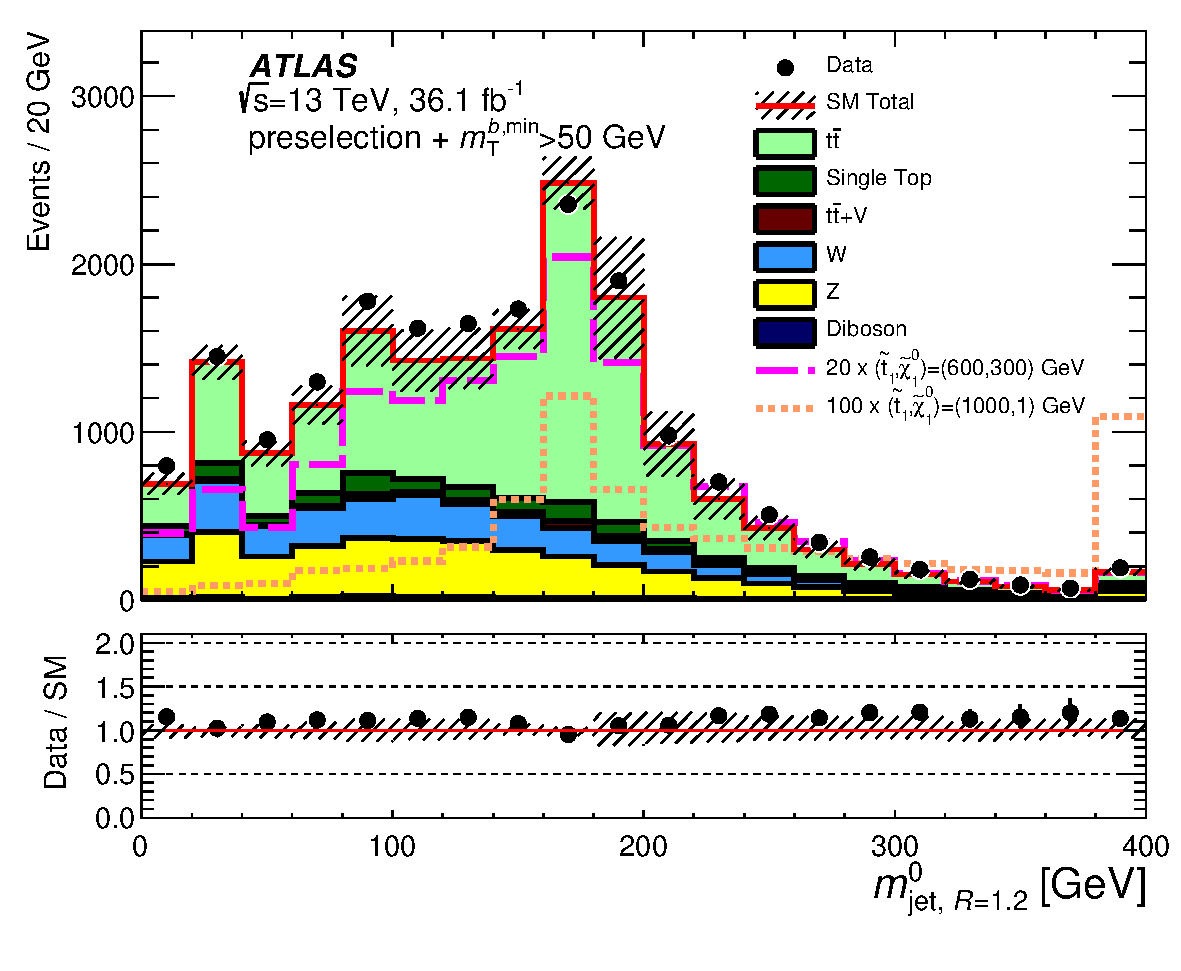
\includegraphics[width=0.48\textwidth]{figures/stop/preselection/AntiKt12M0_preCutSRPlot_withRatio}}
					  \subbottom[]{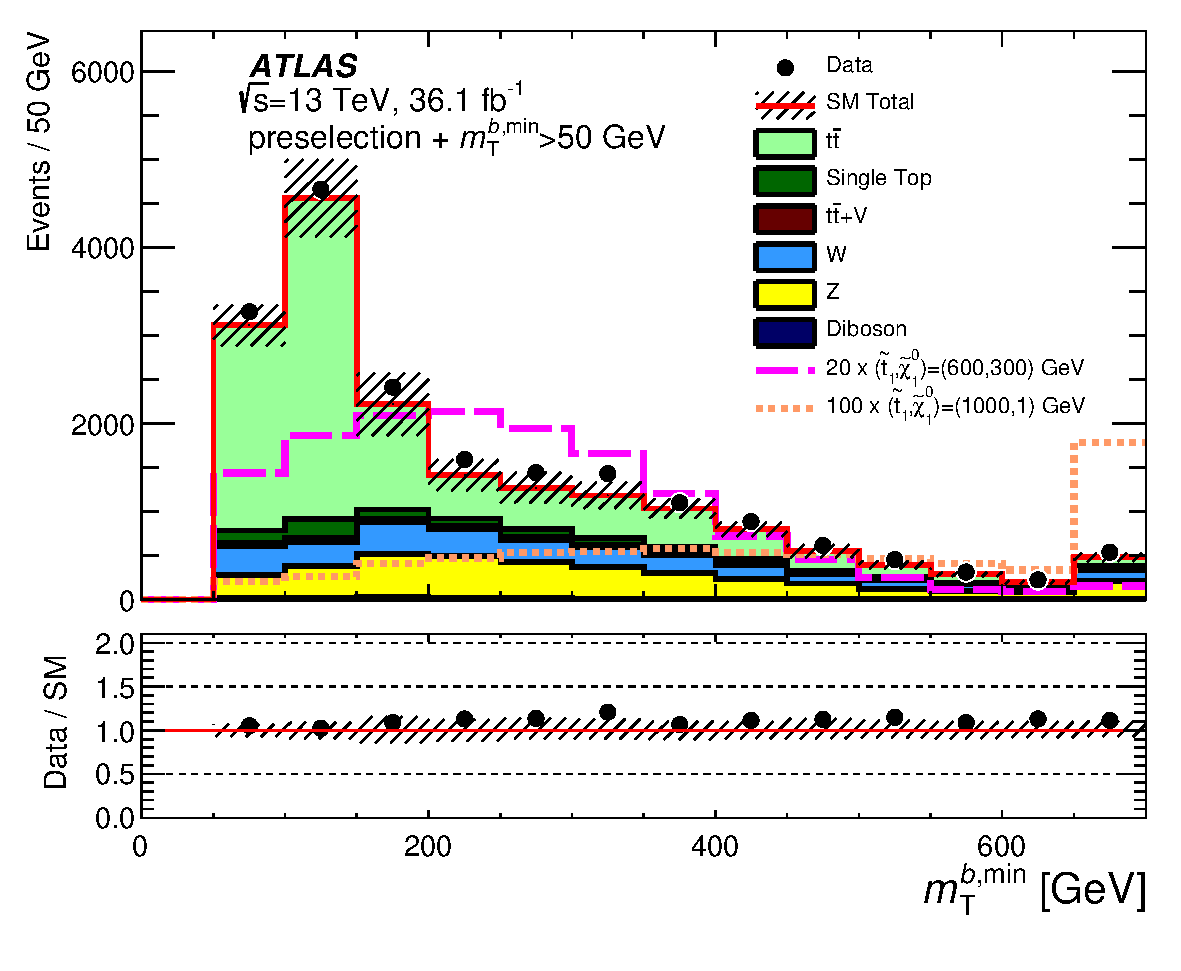
\includegraphics[width=0.48\textwidth]{figures/stop/preselection/MtBMin_preCutSRPlot_withRatio}}
					  \caption{Distributions of the discriminating variables discussed in the text: (a)~\mantikttwelvezero\ and (b)~\mtbmin\ after the pre-selection and an additional $\mtbmin>50\gev$ requirement. The Data/\ac{SM} plots display the ratio of data events to the total \ac{SM} prediction. The band around the \ac{SM} prediction and in the ratio plots illustrates the combination of both statistical and detector-related systematic uncertainties~\cite{stop0L}.}
					  \label{fig:preselection}
				  \end{center}
				\end{figure}

			\paragraph{$\mathbf{\tau}$ veto}

				An additional requirement is applied to reject those events with semi hadronically decaying $\tau$-lepton candidates that are likely to have been yielded from a $\Wboson\to\tau\nu$ decay. In particular, events are rejected when they contain a non-$b$-tagged jet, within $\abseta < 2.5$, with fewer than $4$ tracks associated with it ($\pt > 500$ \MeV), and when the angular difference, in $\phi$, between the jet and \ptmiss\ is less than $\pi/5$. The systematic uncertainties associated to the $\tau$ veto were studied in a paper - to which the author did not contribute -, produced during a previous version of the analysis carried out during Run-1, and were found to be negligible~\cite{stop0LRun1}.



		\subsection{Optimisation strategy}

			The optimisation of \acp{SR} is a fundamental part of every cut-and-count analysis. The goal is to find the best combination of cuts to remove as many background events as possible while retaining the largest possible fraction of signal events. A set of dedicated discriminating variables is therefore employed in each \ac{SR}.

			In order to represent the discovery significance of the signal model targeted, a \ac{FoM} is employed. In counting experiments the significance gives an estimate of the probability that an observed event count in a signal region, could have been produced by the sole fluctuations of the backgrounds in that region. In particular the optimisation of the cuts, of which each \ac{SR} selection is comprised of, is performed by maximising the value of the so-called \Zn\ formula~\cite{Zn}, even though alternative significance definitions can be found on the market~\cite{sigHEP}. The \Zn\ formula, implemented in the \verb+RooStats+~\cite{2010acat.confE..57M} package within the \verb+ROOT+ framework~\cite{Brun:1997pa}, is widely employed in various \ac{SUSY} searches, and it can be written in a simplistic way as it follows: 

			\begin{equation}
				\Zn = \frac{N_\mathrm{sig}}{\sqrt{ N_\mathrm{bkg} + (N_\mathrm{bkg}\sigma_\mathrm{bkg})^2}}
				\label{eq:Zn_forumla}
			\end{equation} 

			\noindent Here, $N_\mathrm{sig}$, $N_\mathrm{bkg}$, and $\sigma_\mathrm{bkg}$ are the signal yields, background yields, and the relative systematic uncertainty on the background, whose value is generally assumed - in a conservative way - a priori. Equation~\ref{eq:Zn_forumla} essentially gives a general idea of what the discovery significance would be, given a certain number of events in a \ac{SR}, the Poisson error on the background $\sqrt{N_{\mathrm{bkg}}}$ and the systematic uncertainty $\sigma_{\mathrm{bkg}N_{\mathrm{bkg}}}$ on the background. Furthermore, there are additional criteria, such as the compatibility with more signal models or a more solid background estimation, that must be followed when \emph{freezing}\footnote{Once all the possible combinations have been investigated and a selection has been agreed upon, the \acp{SR} cuts are fixed in order to move onto performing extensive background studies} a \ac{SR}. The various \ac{SR} selections will then be defined taking into account the above-mentioned criteria combined with the highest value of \Zn. 

			A so-called \emph{blinding} procedure is employed to avoid any potential biases that may affect the analysers during the optimisation of the \acp{SR}. In particular, the number of events - in the collected data - that fall into a signal-enriched region is hidden until the modelling of the backgrounds falling into a \ac{SR} has been solidly tested using background-enriched control (\acp{CR}) and validation regions (\acp{VR}).%\footnote{A procedure employed in many analyses in various disciplines: the number of collected-data events that fall into a signal-enriched region is hidden}
			
			


			\subsubsection*{Signal Regions A and B}

				As already anticipated, SRA and SRB are optimised to target $\stopone \to t + \ninoone$ decays, where the stop-neutralino mass splitting is above the top-quark mass. The fully hadronic $\ttbar$ decay yields six distinct jets and typically they can be reconstructed as six $R=0.4$ \antikt\ jets whose transverse shape is circular with a radius equal to the \antikt\ $R$ parameter. Unfortunately though when the two top quarks are produced with enough boost, precisely when their mutual distance is smaller than $2R$\footnote{in the $\eta$--$\phi$ space}, the top-quark daughter-jet one-to-one correspondence might no longer be true. For this reason the two top candidates are reconstructed by feeding the \antikt\ clustering algorithm~\cite{Antikt2008} with $R=0.4$ jets, using re-clustered radius parameters of $R=0.8$ and $R=1.2$. Two $R=1.2$ re-clustered jets are required and the distribution of the leading $R=1.2$ re-clustered jet mass, for the main backgrounds and the signal, is shown in Figure~\ref{fig:preselection}(a).

				\begin{figure}[!htb]
				  \begin{center}
				   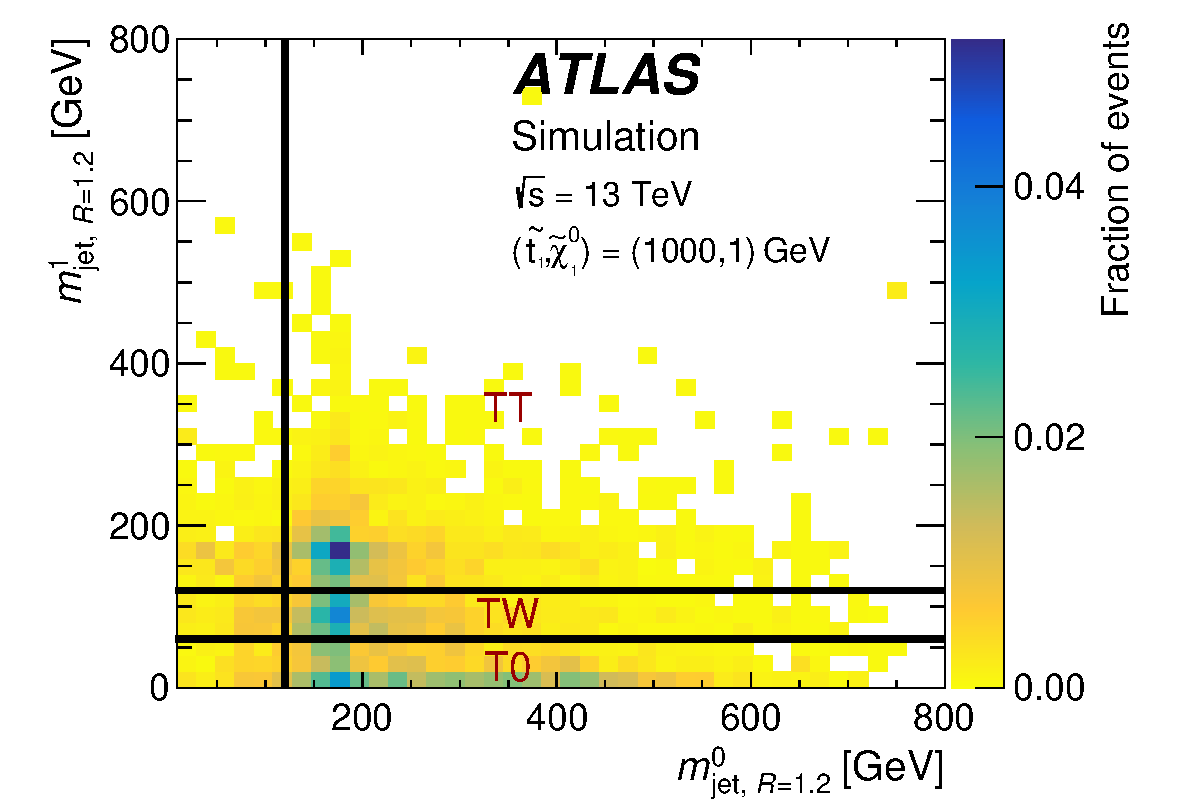
\includegraphics[width=0.7\textwidth]{figures/stop/SRA/CategoryDefs}
				   \caption{2D distribution of \mantikttwelvezero\ and \mantikttwelveone\ top candidate masses to illustrate the signal-region categories (TT, TW, and T0) in simulated direct stop-pair production samples with $(m_{\stop},m_{\ninoone})=(1000,1) \GeV$ after the pre-selection requirement. The black lines represent the requirements on the re-clustered jet masses~\cite{stop0L}.}
				   \label{fig:categories}
				  \end{center}
				\end{figure}

				The main discriminating variables are the re-clustered top masses, with $R = 1.2$ and $R = 0.8$, \mtbmin, \drbb, and \met. Events are grouped into three categories, as shown in Figure~\ref{fig:categories}. The definition of each category is based on the number reconstructed top candidate, as it follows: 
				
				\begin{description}
					\item[TT] includes events with two reconstructed top candidates, namely with masses $\mantikttwelvezero>120\gev$ and $\mantikttwelveone>120\gev$;
					\item[TW] contains events with one reconstructed leading-\pt\ top candidate and one reconstructed sub-leading \Wboson\ candidate from the sub-leading $R = 1.2$ re-clustered mass \ie\ $\mantikttwelvezero>120\gev$ and $60<\mantikttwelveone<120\gev$;
					\item[T0] represents events with only a leading top candidate, \ie\ where $\mantikttwelvezero>120\gev$ and $\mantikttwelveone<60\gev$;
				\end{description}

				\noindent For the benchmark point $(\mstopone, \mninoone) = (1000,1)$ \GeV, after the pre-selection requirements, almost the totality of the events ($\sim 91\%$) fall into the three categories: TT=$38\%$, TW=$22\%$, and T0=$31\%$. Additionally, a  dedicated optimisation on each of such categories, due to differences in kinematics, is performed resulting in the three \acp{SR}, SRA-TT, SRA-TW, SRA-T0, defined in Table~\ref{tab:SRAB}. %Such categories are individually optimised as the signal-over-background ratio varies with them. 
				
				\begin{table}[htb]
				\caption{Selection criteria for SRA and SRB, in addition to the cuts listed in Table~\ref{tab:SRcommon}. SRA and SRB are separated into topological categories based on the number of reconstructed top quarks.}
					\begin{center}
					\renewcommand{\arraystretch}{1.5}
						\begin{tabular}{clccc} \toprule
							{\multirow{2}{*}{\textbf{Signal Region}}}& 			& \multicolumn{3}{c}{\textbf{top Categories}} \\ 
																					&        & {\textbf{TT}}    & {\textbf{TW}}     & {\textbf{T0}}     \\ \toprule%\cline{3-5}%\toprule
							\multirow{4}{*}{{\textbf{A}}} & \mantikteightzero  & \multicolumn{3}{c}{$>60\gev$}        \\ \cline{2-5}
																	& \drbjetbjet        & $>1$        & \multicolumn{2}{c}{-}       \\ \cline{2-5}
																	& \mttwo             & $>400$ \gev  & $>400$ \gev   & $>500$ \gev   \\ \cline{2-5}
																	& \met               & $>400 \gev$ & $> 500 \gev$ & $> 550 \gev$ \\ \midrule
							\multirow{2}{*}{{\textbf{B}}} & \mtbmax            & \multicolumn{3}{c}{$>200\gev$}       \\ \cline{2-5}
																	& \drbjetbjet        & \multicolumn{3}{c}{$>1.2$}                \\\midrule
							\multirow{6}{*}{{\textbf{A and B}}} & \mantikttwelvezero & \multicolumn{3}{c}{$>120\gev$}            \\ \cline{2-5}
																	& \mantikttwelveone  & $>120\gev$  & $[60,120]\gev$ & $<60\gev$  \\ \cline{2-5}
																	& \mtbmin            & \multicolumn{3}{c}{$>200\gev$}            \\ \cline{2-5}
																	& \nBJet    & \multicolumn{3}{c}{$\ge2$}                				\\ \cline{2-5}
																	& $\tau$-veto        & \multicolumn{3}{c}{yes}                   \\ \cline{2-5} 
																	& \dphijetthreemet   & \multicolumn{3}{c}{$>0.4$}                \\ 
																	\bottomrule
						\end{tabular}
					\end{center}
				\label{tab:SRAB}
				\end{table}

				An additional requirement in SRA is on the stransverse mass (\mttwo), especially powerful in the T0 category, as it assumes high values for signals with high top squark and low neutralino masses. \mttwo\ is particularly useful to reconstruct top candidate with lower momenta where the re-clustering was not optimal. Furthermore, in order to maximise the sensitivity to the signal, the top categories are then statistically combined - a logic \verb+OR+ of the three of them is taken - within SRA and SRB.

				Figure~\ref{fig:SRA_bkgcomp} shows the background composition in each of the SRA categories. The main backgrounds are \Zjets\ and \ttV, followed by \ttbar, \Wjets, and single top production. As it will be shown in Section~\ref{sec:bkgest}, dedicated \acp{CR} are used for the TT, TW, and T0 categories, in the regions where enough statistic is present. In particular, for the \Zjets\ background a set of three $2$-lepton \ac{CR} is used, while to control the \ttbar\ and \Wjets\ backgrounds two orthogonal sets of $1$-lepton control regions are used. As the $\ttZ \left ( \to \nu\nu\right)$ is an irreducible background, \ie\ it utterly resembles the signal searched for, its normalisation is instead obtained by using a $1$-lepton-$1$-photon \ttgamma\ \ac{CR}, as it will be shown in~\ref{sec:ddbkgest}.

				\begin{figure}[t]
				  \begin{center}
				   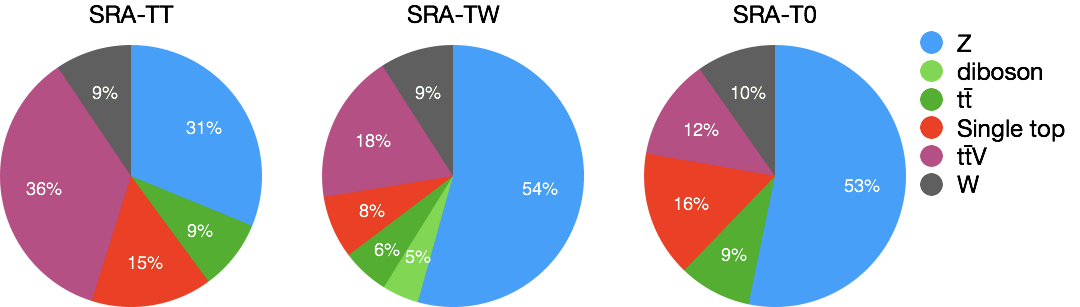
\includegraphics[width=\textwidth]{figures/stop/piechart_SRAcomp}
				   \caption{Background composition in \SRA.}
				   \label{fig:SRA_bkgcomp}
				  \end{center}
				\end{figure}

				For the optimisation of SRB, a similar strategy was adopted. In addition to the \met\ and the re-clustered jet masses, the discriminating variables \mtbmin, \mtbmax, and \drbb\ are employed for the optimisation. After the pre-selection requirement, tightened up by the addition of the requirements of at least two \bjs, $\mtbmin > 200$ \gev, and the tau veto, the fraction of events that fall into the top categories is: TT=$14\%$, TW=20$\%$, T0=$35\%$. The optimal cuts for SRB are also listed in Table~\ref{tab:SRAB}. 

				\begin{figure}[t]
				  \begin{center}
				   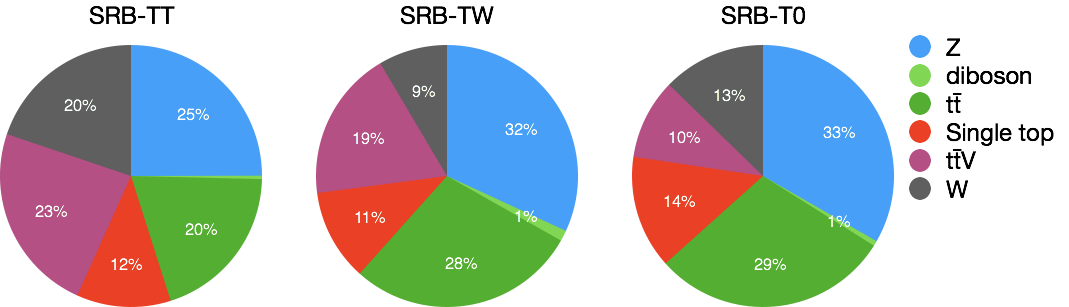
\includegraphics[width=\textwidth]{figures/stop/piechart_SRBcomp}
				   \caption{Background composition in \SRB.}
				   \label{fig:SRB_bkgcomp}
				  \end{center}
				\end{figure}

				Similarly to SRA, Figure~\ref{fig:SRB_bkgcomp} shows the background composition in each of the SRB categories. The dominant backgrounds in SRB are \Zjets\ and \ttbar, with about equal contributions. As already discussed for SRA, the same \acp{CR} are employed to control such dominant backgrounds. The di-boson contributes for less than $1\%$ of the total background therefore no effort will be put in the design of a \ac{CR}. Furthermore, due to the large \met\ requirement, contributions from multi-jet background, are expected to be negligible in both SRA and SRB, nonetheless it will be estimated using the so-called \emph{jet smearing} method~\cite{calumThesis}.




			\subsubsection*{Signal Region C}

				\SRC\ targets a kinematic regime of direct top-squark pair production where the stop-neutralino mass splitting is around the top quark mass. The signature of such decays, when $(\mstopone, \mninoone) \sim m_t$, essentially consists of considerably softer jets and low \met. As it can be seen by looking at the background composition of such \ac{SR} in Figure~\ref{fig:SRC_bkgcomp}, this topology is very similar to a non-resonant \ttbar\ production which makes signal-background separation challenging. Nonetheless the presence of \ac{ISR} can help exploit kinematical differences between stop decays and \ttbar\ production. In particular, when the event is characterised by the presence of a high-momentum \ac{ISR} - reconstructed as an \ac{ISR} system formed by multiple jets - the system comprised of the two top-squarks is produced with a boost in the transverse plane.

				\begin{figure}[t]
				  \begin{center}
				   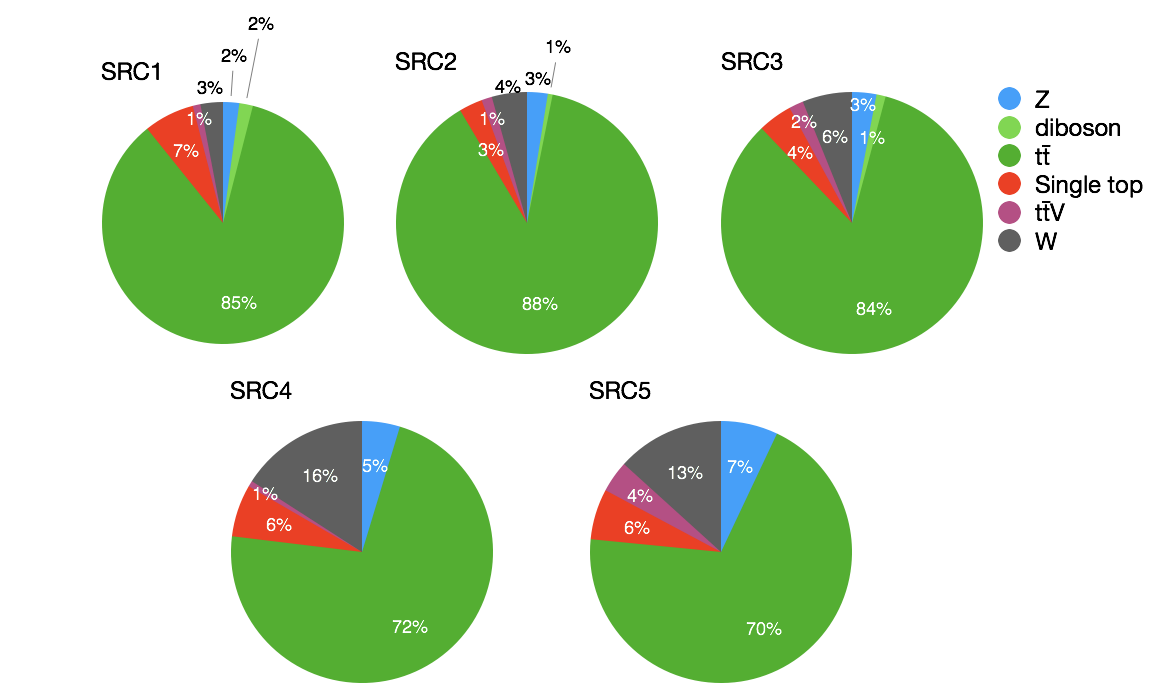
\includegraphics[width=\textwidth]{figures/stop/piechart_SRCcomp}
				   \caption{Background composition in \SRC.}
				   \label{fig:SRC_bkgcomp}
				  \end{center}
				\end{figure}

				A new dedicated set of variables can be defined employing the so-called \emph{\ac{RJR}} of which a brief overview is given. Such technique is used to divide each event into hemispheres: an \ac{ISR} and a sparticle hemisphere. The latter is comprised of a pair of top-squark candidates both decaying via $t + \ninoone$. Objects are grouped together based on their proximity in the lab frame's transverse plane by minimizing the reconstructed transverse masses of the \ac{ISR} system and sparticle system simultaneously over all choices of object assignment. A dedicated set of kinematic variables is then defined, based on this assignment of objects to either the \ac{ISR} system or the sparticle system. This method is equivalent to grouping the event objects according to the axis of maximum back-to-back \pt\ in the event's \ac{CM} frame where the vectorial sum of all the \pt\ of the accepted objects is zero. In events with a high-\pT\ \ac{ISR} gluon, the axis of maximum back-to-back \pt\ approximates the direction of the \ac{ISR} and sparticles' back-to-back recoil. Additional details on such technique can be found in Ref.~\cite{RJR_ISR}.
				\begin{table}[htpb]
				  \caption{Selection criteria for SRC, in addition to the pre-selection listed in Table~\ref{tab:SRcommon}. The \acp{SR} are separated into $\RISR$-based windows.}
				  \begin{center}
				    \def\arraystretch{1.5}
				    \begin{tabular}{lccccc} \toprule
				      {\textbf{Selection}} & \textbf{SRC1} & \textbf{SRC2} & \textbf{SRC3} & \textbf{SRC4} & \textbf{SRC5} \\ \toprule
				      \rISR & 0.30--0.40 & 0.40--0.50 & 0.50--0.60 & 0.60--0.70 & 0.70--0.80\\ \midrule %\midrule \hline
				      \nBJet & \multicolumn{5}{c}{$\ge1$} \\ %\hline
				      \nBJetS & \multicolumn{5}{c}{$\ge1$} \\ %\hline
				      \nJetS & \multicolumn{5}{c}{$\ge5$}  \\ %\hline
				      \pTSBZero & \multicolumn{5}{c}{$>40\gev$}  \\ %\hline
				      \mS & \multicolumn{5}{c}{$>300\gev$}  \\ %\hline
				      \dPhiISRMET & \multicolumn{5}{c}{$>3.0$}  \\ %\hline
				      \pTISR & \multicolumn{5}{c}{$>400$ \gev}   \\ %\hline
				      \pTSFour & \multicolumn{5}{c}{$>50$ \gev}   \\ \bottomrule
				    \end{tabular}
				  \end{center}
				  \label{tab:SignalRegionC}
				\end{table}

				The ratio of the \met\ to the \pt\ of the \ac{ISR} system in the \ac{CM} frame of the entire (\ac{ISR} plus di-top-squark) system (\pTISR), defined as \rISR, is proportional to the ratio of the $\ninoone$ and $\stop$ masses and it is defined as it follows~\cite{An,Macaluso}:
				
				\begin{equation*}
					\rISR \equiv \frac{\met}{\pTISR} \sim \frac{m_{\ninoone}}{m_{\stop}}. 
				\end{equation*}

				\noindent Additionally, the following discriminating key variables are used in the optimisation of SRC: 

				\begin{description}
					\item[\boldmath \nBJetS:] number of \bjs\ associated with the sparticle hemisphere;
					\item[\boldmath \nJetS:] number of jets associated with the sparticle hemisphere;
					\item[\boldmath \pTSBZero:] \pt\ of the leading \bj\ in the sparticle hemisphere;
					\item[\boldmath \pTSFour:] \pt\ of the fourth-leading jet in the sparticle hemisphere;
					\item[\boldmath \dPhiISRMET:] angular separation in $\phi$ of the \ac{ISR} and the \met\ in the \ac{CM} frame;
					\item[\boldmath \pTISR:] \pt\ of the \ac{ISR} system, evaluated in the \ac{CM} frame;
					\item[\boldmath \mS:] transverse mass between the whole sparticle system and \met;
					\item[\boldmath \mV/\mS:] ratio of the transverse mass of the only the visible part of the sparticle system without \met and the whole sparticle system including \met;
				\end{description}				

				Table~\ref{tab:SignalRegionC} lists the selection criteria for SRC. Five different non-overlapping \RISR-based sub regions (windows) are employed, each of which targets different signal points, \eg\ SRC2 is optimised for $(\mstop, \mninoone) = (300,127) $ \GeV; SRC4 is optimised for $(\mstop, \mninoone) = (500,327)$. Additionally, a minimum of five jets are required to be assigned to the sparticle hemisphere of the event (\nJetS), and at least one of them (\nBJetS) must be $b$-tagged. Requirements on \pTISR, the highest-\pt\ \bj\ in the sparticle hemisphere (\pTSBZero), and the fourth-leading jet in the sparticle hemisphere (\pTSFour), are also applied. Furthermore, the transverse mass built from the sparticle system and the \met\ (\mS), is required to be above $300\GeV$. Finally, the angular distance in $\phi$ between the \ac{ISR} system and the \ptmiss\ in the \ac{CM} frame is required to be above $3$. As with SRA and SRB, the five $\RISR$ windows are statistically combined to improve signal sensitivity.





			\subsubsection*{Signal Region D}

				%\begin{table}[!htb]
				\begin{wraptable}{R}{.5\textwidth}
				  \caption{Selection criteria for SRD, in addition to the common pre-selection shown in Table~\ref{tab:SRcommon}.}
				  \begin{center}
				  \def\arraystretch{1.4}
				  \begin{tabular}{lcc}
				    \toprule
				    {\textbf{Selection}}       & {\textbf{SRD-low}} & {\textbf{SRD-high}} \\
				    \toprule
				    \dphijetthreemet     & \multicolumn{2}{c}{$>0.4$}     \\ %\hline
				    \nBJet      & \multicolumn{2}{c}{$\geq$2}    \\%\hline
				    \drbjetbjet     & \multicolumn{2}{c}{$>$ 0.8}    \\ %\hline
				    \ptbzero+\ptbone & $>300$ \gev    & $>400$ \gev     \\ %\hline
				    $\tau$-veto          & \multicolumn{2}{c}{yes}        \\ %\hline
				    \ptone\              & \multicolumn{2}{c}{$>150\GeV$} \\ %\hline
				    \ptthree\            & $>100\GeV$    & $>80\GeV$      \\ %\hline
				    \ptfour\             & \multicolumn{2}{c}{$>60\GeV$}  \\ %\hline
				    \mtbmin\             & $>250\GeV$    & $>350\GeV$     \\ %\hline
				    \mtbmax\             & $>300\GeV$    & $>450\GeV$     \\ 
				    \bottomrule
				  \end{tabular}
				  \end{center}
				  \label{tab:SignalRegionD}
				\end{wraptable}
				\SRD\ targets direct top-squark pair production where both top squarks decay via $\stop\to b \chinoonepm$ and the chargino mass is set to be $m_{\chinoonepm}=2\mLSP$, therefore a nominal signature of six jets, two of which $b$-tagged. In this \ac{SR} no top-quark reconstruction is needed. 

				SRD is divided into two sub-regions, SRD-low and SRD-high, which are optimised for $\mstop = 400\GeV$ with $\mLSP=50\GeV$, and $\mstop = 700\GeV$ with $\mLSP=100\GeV$, respectively. As it can be seen in Figure~\ref{fig:SRD_bkgcomp} the main backgrounds in SRD are \Zjets\ and \Wjets. The production of \ttbar, together with single top, and \ttV\ yield around the same number of events.

				\begin{figure}[t]
				  \begin{center}
				   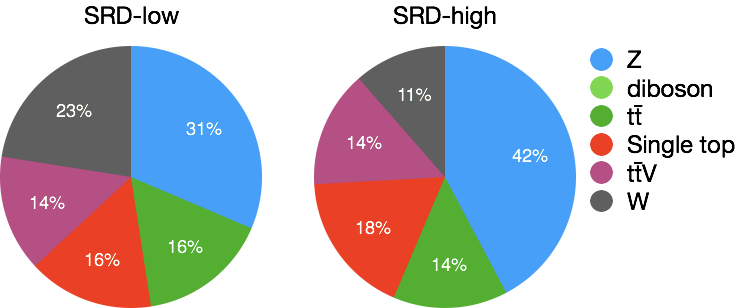
\includegraphics[width=.7\textwidth]{figures/stop/piechart_SRDcomp}
				   \caption{Background composition in \SRD.}
				   \label{fig:SRD_bkgcomp}
				  \end{center}
				\end{figure}

				In this \ac{SR}, at least five jets are required, two of which must be $b$-tagged. As previously anticipated, a cut on the distance between the two jets with the highest MV2c10 weights is required to reject event with two \bjs\ originated from gluon splitting. On top of the discriminating variables already discussed for the other \ac{SR}, the scalar sum of the transverse momenta of the two jets with the highest MV2c10 weights (\ptbzero+\ptbone) together with the second (\ptone), fourth (\ptthree), and fifth (\ptfour) jet transverse momenta, are used as discriminating variables to provide further background rejection. Finally, tighter requirements on the leading and sub-leading jet $\pT$ are made for SRD-high. Table~\ref{tab:SignalRegionD} shows a summary of SRE selection.






			\subsubsection*{Signal Region E}


				Unlike the previous \acp{SR}, as mentioned in Section~\ref{sec:susysig}, SRE is designed for signal models in which top quarks are produced highly boosted. The scenarios targeted by this \ac{SR} can arise from either direct pair production of high-mass stop quarks, or from the gluino-mediated compressed stop production with a large gluino-stop mass splitting. In this regime, re-clustered jets with $R=0.8$ are employed for the optimisation of the experimental sensitivity to such highly boosted top quarks. In particular, the signal point used for the optimisation is $m_{\gluino} = 1700 \GeV$, $\mstop=400\GeV$, and $\mLSP=395\GeV$

				Figure~\ref{fig:SRE_bkgcomp} shows the background composition in SRE. The main backgrounds are \Zjets\ and \ttV\ followed by single top, \Wjets, and \ttbar\ production. A dedicated $2$-lepton \Zjets\ \ac{CR} is employed for the normalisation of such background.  In this \ac{SR}, at least two jets out of the four or more required jets must be $b$-tagged. Additional discrimination is provided by the $\met$ significance: $\htsig$, where $\HT$ is the scalar sum of the $\pT$ of all the reconstructed $R=0.4$ jets in the event. The selection criteria for SRE, optimised for $m_{\gluino} = 1700 \GeV, \mstop=400\GeV$, and $\mLSP=395\GeV$, are listed in Table~\ref{tab:SignalRegionE}.

				\begin{figure}[!htb]
					\centering
					\begin{minipage}[]{.5\textwidth}
						\centering
						\vspace{0pt}
						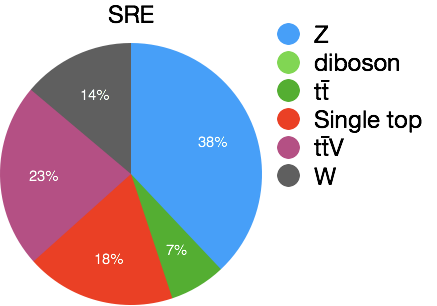
\includegraphics[width=\textwidth]{figures/stop/piechart_SREcomp}
						\caption{Background composition in \SRE.}
						\label{fig:SRE_bkgcomp}
					\end{minipage}\hfill
					\begin{minipage}[!htb]{.5\textwidth}
						\centering
						\vspace{0pt}
						% \begin{table}
						\def\arraystretch{1.4}
						\captionof{table}{Selection criteria for SRE in addition to the common pre-selection cuts listed in Table~\ref{tab:SRcommon}}
							\begin{tabular}{lc}\toprule
							   {\textbf{Selection}}    & {\textbf{SRE}}\\
							   \toprule
							   \dphijetthreemet  & $>0.4$             \\ %\hline
							   \nBJet   & $\geq$2            \\     %\hline
							   \mantikteightzero & $>120$ \gev        \\     %\hline
							   \mantikteightone  & $>80$ \gev         \\     %\hline
							   \mtbmin\          & $>200$ \gev        \\     %\hline
							   \met\             & $> 550 \gev$       \\     %\hline
							   \HT               & $>800 \gev$        \\     %\hline
							   \htsig            & $> 18 \sqrt{\GeV}$ \\     
							   \bottomrule
							   \label{tab:SignalRegionE}
							\end{tabular}
						% \end{table}
					\end{minipage}
				\end{figure}

